%%%%%%%%%%%%%%%%%%%%%%%%%%%%%%%%%%%%%%%%%%%%%%%%%%%%%%%%%%%%%%%%%%%%%%%%%%%%%%%%
%2345678901234567890123456789012345678901234567890123456789012345678901234567890
%        1         2         3         4         5         6         7         8
% DOCUMENT CLASS
\documentclass[oneside,12pt]{Classes/RoboticsLaTeX}

% USEFUL PACKAGES
% Commonly-used packages are included by default.
% Refer to section "Book - Useful packages" in the class file "Classes/RoboticsLaTeX.cls" for the complete list.
\usepackage{amsmath}
\usepackage{amsfonts}
\usepackage{algorithm}
\usepackage{algorithmic}
\usepackage{multirow}
\usepackage{colortbl}
\usepackage{color}
\usepackage[table]{xcolor}
\usepackage{epigraph}
\usepackage{graphicx}
%\usepackage{subfigure}
\usepackage{caption}
\usepackage{subcaption}
\usepackage{hyperref}
\usepackage{varioref}
% \usepackage{cleveref}
\usepackage{tabularx}
\usepackage{caption}
\usepackage{float}
\usepackage{longtable}
\usepackage[pdftex]{graphicx}
\usepackage{pdfpages}
%\usepackage{tabularx}
\usepackage{pdflscape}
\usepackage[acronym,toc]{glossaries}
\usepackage{setspace}
\setstretch{1.5}
%\onehalfspacing
\usepackage{minted}
% SPECIAL COMMANDS
% correct bad hyphenation
\hyphenation{op-tical net-works semi-conduc-tor}
\hyphenation{par-ti-cu-lar mo-du-le ge-stu-re}
% INTERLINEA 1.5
%\renewcommand{\baselinestretch}{1.5}

%% ignore slightly overfull and underfull boxes
%\hbadness=10000
%\hfuzz=50pt
% declare commonly used operators
\DeclareMathOperator*{\argmax}{argmax}

% HEADER
\ifpdf
    \pdfinfo {/Title (Bachelor thesis on LoRaWan)
              /Creator (TeX)
              /Producer (pdfTeX)
              /Author (Pablo Salinas, Javier Pardiño, Iñigo García)
              /CreationDate (D:20220628000000) %format D:YYYYMMDDhhmmss
              /ModDate (D:2022062800000)
              /Subject (On the LoRaWan technologies: a case study of Genova)
              /Keywords (Bachelor, Thesis)}
    \pdfcatalog {/PageMode (/UseOutlines)
                 /OpenAction (fitbh) }
\fi

\title{\Large{Empirical study of LoRaWan on the study case of Genova}}

\ifpdf
  \author{Pablo Salinas, Javier Pardiño, Iñigo García
          }
  \collegeordept{}
  \university{Public University of Navarre \& University of Genova}
  \crest{
\includegraphics[width=40mm]{logo_upna.jpeg} \includegraphics[width=30mm]{logo_unige}}
\else
  \author{Pablo Salinas, Javier Pardiño, Iñigo García
          }
  \collegeordept{}
  \university{Public University of Navarre \& University of Genova}
  \crest{
\includegraphics[width=40mm]{logo_upna.jpeg} \includegraphics[width=30mm]{logo_unige}}
\fi
% nome relatore tesi 
\supervisor{Daniele Caviglia}

% DECLARATION
% Use the following command to change the declaration text:
\newcommand{\code}{\texttt}
\renewcommand{\submittedtext}{In the bachelor's thesis for the}
\degree{Degree of Telecomunications Engineering; international variant}
\degreedate{June 28, 2022}
\hypersetup{
    urlcolor=cyan,
    }
%%%%%%%%%%%%%%%%%%%%%%%%%%%%%%%%%%%%%%%%%%%%%%%%%%%%%%%%%%%%%%%%%%%%%%%%%%%%%%%%
\makeglossaries
\loadglsentries{glossary}

\begin{document}

% A page with the abstract and running title and author etc may be
% required to be handed in separately. If this is not so, comment
% the following 3 lines:
% \begin{abstractseparate}
%   %        1         2         3         4         5         6         7         8
% THESIS ABSTRACT

% Use the following style if the abstract is long:
%\begin{abstractslong}
%\end{abstractslong}

\begin{abstracts}

This thesis aims to:
\begin{itemize}
    \item Mesure performance LoRaWan comunication standard on packed cities and with moving end nodes
    \item Many different scenarios were tested and analized
    \item The conclusions reached prove that the asumptions made were sound
\end{itemize}

\end{abstracts}

% \end{abstractseparate}
\begin{spacing}{1}
\maketitle
\end{spacing}

% add an empty page after title page
\newpage\null\thispagestyle{empty}\newpage

% set the number of sectioning levels that get number and appear in the contents
\setcounter{secnumdepth}{3}
\setcounter{tocdepth}{3}


\frontmatter
%%%%%%%%%%%%%%%%%%%%%%%%%%%%%%%%%%%%%%%%%%%%%%%%%%%%%%%%%%%%%%%%%%%%%%%%%%%%%%%%%
%2345678901234567890123456789012345678901234567890123456789012345678901234567890
%        1         2         3         4         5         6         7         8
% THESIS ACKNOWLEDGEMENTS

% Use the following style if the acknowledgements are long:
%\begin{acknowledgementslong}
%\end{acknowledgmentslong}

\begin{acknowledgements}


%“I don't know half of you half as well as I should like; and I like less than half of you half as well as you deserve.”
 %J.R.R. Tolkien, The Fellowship of the Ring 

Write here your acknowledgements...


\end{acknowledgements}

%        1         2         3         4         5         6         7         8
% THESIS ABSTRACT

% Use the following style if the abstract is long:
%\begin{abstractslong}
%\end{abstractslong}

\begin{abstracts}

This thesis aims to:
\begin{itemize}
    \item Mesure performance LoRaWan comunication standard on packed cities and with moving end nodes
    \item Many different scenarios were tested and analized
    \item The conclusions reached prove that the asumptions made were sound
\end{itemize}

\end{abstracts}


\tableofcontents
\listoffigures
\listoftables
\printglossary[title=List of Acronyms,type=\acronymtype]
%\printglossary  % Print the nomenclature (WAY TOO COMPLEX FOR ME NOW!)
%\addcontentsline{toc}{chapter}{Nomenclature}

\mainmatter
%%%%%%%%%%%%%%%%%%%%%%%%%%%%%%%%%%%%%%%%%%%%%%%%%%%%%%%%%%%%%%%%%%%%%%%%%%%%%%%%
%2345678901234567890123456789012345678901234567890123456789012345678901234567890
%        1         2         3         4         5         6         7         8
% THESIS INTRODUCTION

\chapter*{Introduction}
\label{chap:introduction}
\ifpdf
    \graphicspath{{Introduction/Figures/PNG/}{Introduction/Figures/PDF/}{Introduction/Figures/}}
\else
    \graphicspath{{Introduction/Figures/EPS/}{Introduction/Figures/}}
\fi

% quote

%\setlength{\epigraphwidth}{.35\textwidth}
%\epigraph{Research is formalized curiosity.}{ Zora Neale Hurston, 1942}

% examples of sections

\section{Motivations}
\label{motivations}
In recent years, Internet Of Things technologies (IoT) have grown in
importance and are expected to have an exponential increase in their
use in the coming years. For this reason, there is a need for
communication protocols with two key features, which are:
- Long range communications
- Low power consumption.
To cover these needs LPWANs (Low Power Wide Area Networks) were
created and offer big advantages when compared to high bitrate and
shorter range technologies such as Wi-Fi or Bluetooth, and cellular ones
like GSM or 4G that have a much higher power consumption.\\
The study of these technologies on the enviroment of tightly packed 
cities is highly important in order to advance to achive smart cities.
  
\section{Context of the Study}
\label{context}
The study is performed on the city of Genova, thightly packed with 
buildings, for the most part made with concrete and brick. Other 
cities with different architecture could perform different as the 
distribution of the buildings is important in the reach of the 
signal. One example of this is the problems with GPS localization 
when near skyscrapers.

\section{Tools used in the thesis}
\label{objectives}
For the storage and analysis of these messages The Things Network is
being used, which is a free to use LoRa network that offers not only
gateways but also data storage and various functionalities for a
particular network, being able to make it private or public.

\section{Overview of the Thesis}
\label{overview}
In this thesis we are going to take a look at LoRaWAN (Long Range
Wide Area Network), a communication protocol with a low bit rate and
power consumption that can reach distances of up to several kilometres,
we will study the characteristics of the communication and recreate
various real life scenarios to study different characteristics such as
packet loss, power transmitted and the best configuration for the end-
devices. With these measurements we can obtain valuable information
about how to optimize the network for its different use cases, as there
are big differences depending on the topology and placements of the
nodes and gateways.
%%%%%%%%%%%%%%%%%%%%%%%%%%%%%%%%%%%%%%%%%%%%%%%%%%%%%%%%%%%%%%%%%%%%%%%%%%%%%%%%
%2345678901234567890123456789012345678901234567890123456789012345678901234567890
%        1         2         3         4         5         6         7         8
% THESIS Chapter

\chapter{Previous required knowledge}
\label{chap:first}
\ifpdf
    \graphicspath{{Chapter1/Figures/PNG/}{Chapter1/Figures/PDF/}{Chapter1/Figures/}}
\else
    \graphicspath{{Chapter1/Figures/EPS/}{Chapter1/Figures/}}
\fi


\section{LPWAN}
\label{sec:f-lpwan}
LoRa and LoRaWAN protocols are based on the LPWAN technology.
LPWAN stands for “Low Power Wide Area Network” and it allows radio-
equipped devices to communicate more efficiently and over longer
distances. This emergent technology had the goal of finding a better
data transmission protocol than other technologies such as Bluetooth,
Wi-Fi or 3G/4G. The low-power consumption and the long range
transmission that this technology offers, positions it as a cost-effective
solution when compared with the other big technologies. As LPWAN is
not concerned with transmitting big quantities of data, it offers aspects
that simply others can't complete such as the coverage of long distances
as it can be appreciated in the figure below.
\begin{figure}[htbp]
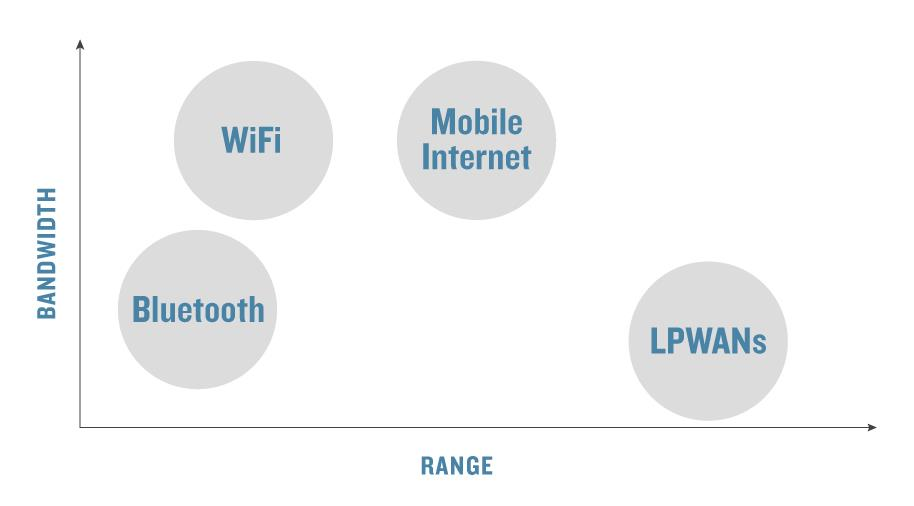
\includegraphics[width=\linewidth]{rangevsband.png}
\caption{Graph comparison of range and bandwidth for different data transmission technologies.}
\end{figure}

This is why LPWAN has become one of the fastest growing spaces in
the Internet of Things (IoT) ecosystem. One of the biggest and most
interesting applications of this data transmission technology is on the
Smart Cities field. This protocols are a perfect solution for the Smart City
data networks, which requires low data rate but constant data streams
and the coverage of long distances with the benefit of using significantly
less power than other data network platforms. Shanghai is a perfect
example of a Smart City where LPWAN is used in order to connect
thousands of sensors to measure the air quality and human movement, more info 
\href{https://www.citiesforum.org/news/what-made-shanghai-the-worlds-no-1-smart-city}{here}.
The future of this technology is bright as IoT devices are growing a 12\%
annually according to a \href{https://cdn.ihs.com/www/pdf/IoT_ebook.pdf}{IHS Markit report}.
and LPWAN is one of the greatest spaces in the IoT ecosystem. LoRa and LoRaWAN are
realizations of the Low Power WAN concept, and with such high demand
for the technology both are having great impulse in their development.
\section{LoRa}
\label{sec:f-lora}
LoRa is the protocol which defines the physical (radio) layer of the
communications in \acrfull{ttn}. This protocol fixes the
frequency band and defines the modulation that is used to transmit data
which enables the long-range communication link.\\
The frequency band depends on the region in which you are, for
example, in the US they use a band from 902.3 to 914.9 MHz, here in
Europe the band goes from 863 to 870 MHz as it's ilustrated on the next table:\\

\begin{table}[htbp]
\centering
\setlength{\arrayrulewidth}{0.5mm}
\setlength{\tabcolsep}{18pt}
\renewcommand{\arraystretch}{2}
\begin{tabular}{ |p{5cm}|p{5cm}| }
\hline
\multicolumn{2}{|c|}{\cellcolor[HTML]{85C1E9}Frequency band depending on the region } \\
\hline
\cellcolor[HTML]{AED6F1} Region & \cellcolor[HTML]{AED6F1} Frequency (Mhz) \\
\hline
Asia & 433  \\
Europe & 863-870 \\
US & 902-928 \\
Australia & 915-918  \\
Canada & 779-787  \\
China & 470-510  \\
\hline
\end{tabular}
\caption{frequency band of different regions}
\end{table}

The LoRa modulation is based on the Spread Spectrum technique and
it's crucial for the long distance communication. This technique spreads
the signal all over the frequency band and it allows LoRa to be very
robust to interferences and noise, allowing the signal to reach longer
distances. More precisely it's called chirp modulation and it transmits
symbols encoding them into multiple signals of increasing (upchirp) or
decreasing (downchirp) radio frequencies. A LoRa transmission always
starts with 8 upchirps and 2 downchirps as we can see in the figure
number 1.2.
\begin{figure}[htbp]
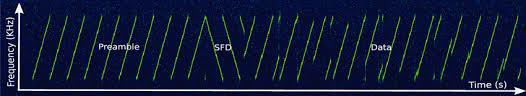
\includegraphics[width=\linewidth]{lorainitchirp.png}
\caption{Snapshot of a LoRa transmission}
\end{figure}
In LoRa communications we are able to reduce our data rate in order to
gain range by changing the Spreading Factor. The Spreading Factor
means the number of raw bits that can be encoded in a symbol.
(“Modelling and Performance Evaluation of LoRa Network Based on
Capture ...”) The \acrfull{sf} value goes from 7 to 12 and as we increase this
value the number of raw bits in a symbol increase and this leads to a
gain of range but also to a reduction of data rate, to an incrementation
of the time on air and to more battery consumption. \\
The SF value can vary from 7 to 12 both included, trading data rate with
range. The increase or decrease in data rate is proportional to the time
on air, greater meaning not only more battery consumed but also greater
chance of collision. The increase in range is due to the higher sensitivity
of the receiver at greater values of SF. In short, increasing a level the
SF means stretching the signal twofold, with its corresponding higher
power consumption but better range.\\
LoRa has to deal with the specific regulations and norms of each region.
Here in Europe we must comply the following rules:
\begin{itemize}
   \item For uplink, the maximum transmitted power is limited to 25 mW
(14dBm) 
    \item For downlink, the maximum transmission power is limited to 0.5W
(27dBm)
    \item There is between an 0.1\% and 1\% duty cycle per day. This means
            that the time on air of the transmission must not exceed a
            proportion of the total time.
    \item Maximum allowed antenna gain +2.15 dBi
\end{itemize}
\section{TTN and LoRaWAN}
\label{sec:f-ttnandlora}
LoRaWAN defines the communication protocol and the system
architecture, it acts like a MAC layer for LoRa packets. The Things
Network is a LoRaWAN network operator that use this protocol and its
network topology to give free LoRaWAN connectivity. \\
The LoRaWAN network topology, as it's represented in figure 1.3,
consist of 4 layers: end-nodes, gateway, network server and application
server.
\begin{figure}[htbp]
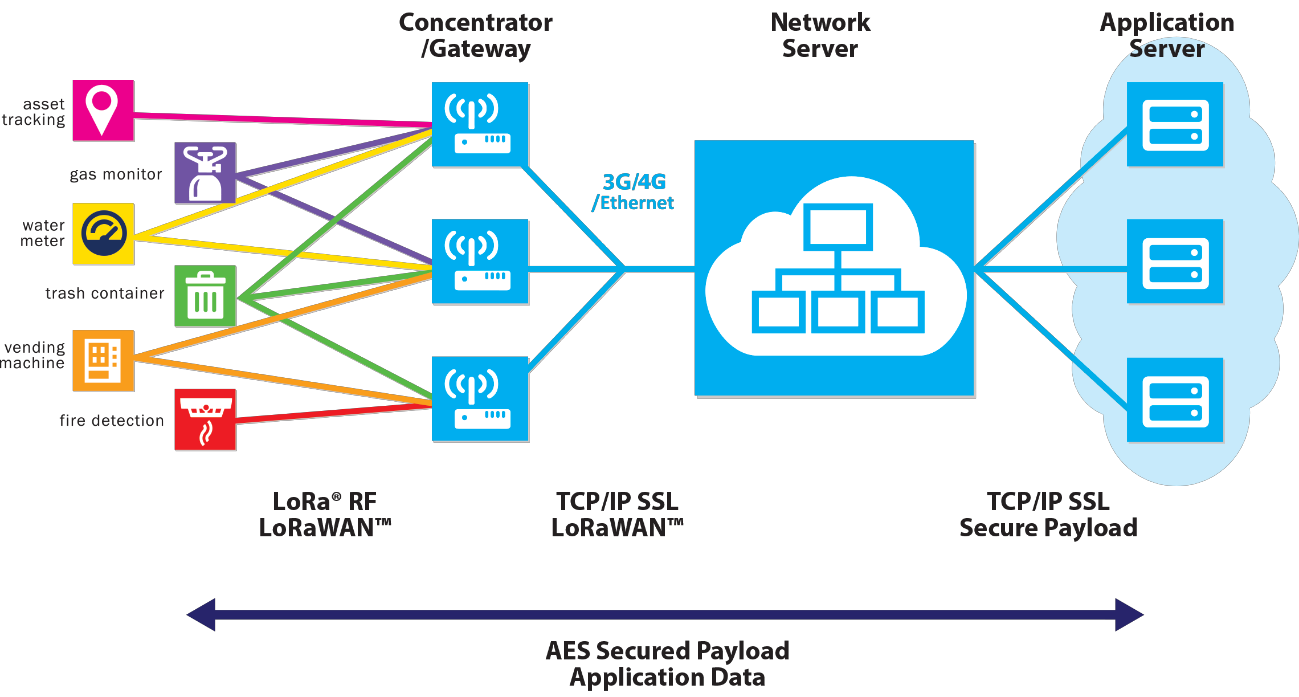
\includegraphics[width=\linewidth]{ttnarch.png}
\caption{LoRaWAN network topology}
\end{figure}
Gateways are able to listen from hundreds of end nodes at the same
time, even if those nodes are transmitting at different frequencies or SF.
The data transmitted through the gateways arrives to the network server
via TCP/IP. Then the network server (NS) sends those packets to the
application server (AS) and if it is needed, a different server called join
server (JS), enters in the process. This server stores the sensitive parts
of LoRaWAN applications such as the root keys and generates the
session keys when a join procedure takes place.\\
In LoRaWAN communications we distinguish two types of transmissions
depending on the sense of communication. An uplink message is sent
from an end-node to a network server and in the case of a downlink
message the message in sent from a network server to a specific device.

\begin{itemize}
    \item \textbf{Uplink message:} this message uses the 
    LoRa radio packet explicit mode, which consists of a physical 
    header (PHDR) and a cyclic redundancy check (CRC) header (PHDR-CRC). 
    Another CRC is required to protect the integrity of the payload; all of
    them are together inserted by the radio transciver in the following way:
    \begin{center}
    \begin{tabular}{ |c|c|c|c|c| } 
     \hline
     Preamble & PHDR & PHDR-CRC & PHYPayload & CRC\\ 
     \hline
    \end{tabular}
    \captionof{table}{Uplink message format.}
    \end{center}
    
    \item \textbf{Downlink message:} The structure is very similar to the uplink message, the only difference is that in a downlink message there is no existence of CRC:
    \begin{center}
    \begin{tabular}{ |c|c|c|c| } 
     \hline
     Preamble & PHDR & PHDR-CRC & PHYPayload \\ 
     \hline
    \end{tabular}
    \captionof{table}{Downlink message format.}
    \end{center}
\end{itemize}
    
This PHYPayload that both, the uplink and the downlink messages contains, starts with a single-octet MAC header (MHDR), followed by a MAC payload (MACPayload) and finishing with a 4-octet message
integrity code (MIC):
\begin{center}
\begin{tabular}{ |c|c|c| } 
    \hline
    MHDR & MACPayload & MIC \\ 
    \hline
\end{tabular}
\captionof{table}{PHYPayload}
\end{center}

The MHDR defines the type of the message that is sent. Those types are join request, join accept, unconfirmed data up/down and confirmed data up/down, where confirmed means that it has to be acknowledged by the receiver, while unconfirmed does not require that.

The MACPayload contains a frame header (FHDR), which is the device address of an end-device (DevAddr), followed by an optional port field (FPort) and an optional frame payload field (FRMPayload):

\begin{center}
\begin{tabular}{ |c|c|c| } 
    \hline
    FHDR (DevAdd) & FPort & FRMPayload \\ 
    \hline
\end{tabular}
\captionof{table}{MACPayload}
\end{center}

Three device classes are defined in LoRaWAN:
\begin{itemize}
    \item Class A: in this class after the uplink transmission two reception
windows are set in order to receive downlink messages. A stands
for All, since all devices must implement this functionality.
    \item Class B: in addition to class A devices, this class open extra
receive windows at scheduled times. Time synchronized beacons
are sent from the gateway to fix those scheduled times in the end
node.
    \item Class C: this type of devices have almost all time open receive
windows and are only closed when transmitting.
\end{itemize}
Class A is the most common class as it is the most energy efficient.\\
The frequency band defined by LoRa is divided into 8 channels. In the
case of downlink messages there are 8 channels used by the first
reception window and another one used by the second window. Due to
the regulations in Europe each channel must be of 125 KHz of
bandwidth. During a data transmission the channel is constantly
changing in order to make the communication more robust to
interferences.\\
An important mechanism that is used to control the uplink connection
between the end node and the gateway is the \acrfull{adr}. This protocol is able to modify automatically parameters like the
Spreading Factor or the transmission power according to the signal
power that the gateway is receiving. As it's explained before, the SF also
affects the power used by the node so this mechanism is able to find the
optimal point in which the node is only using the necessary power. The
Things Network allows to disable or enable it depending on your
purpose. If the device is stationary, TTN recommends to leave the ADR
active, but if the end node is supposed to move, the SF and power
should be in charge of the programmer.\\
The ADR algorithm is simple, but has important ramifications on 
the performance if the device is not stationary.
The reason for this is that the ADR algorithm was designed in order
to provide the best bandwidth utilization and the best battery life
to devices with an stable radio communication. From this falls that 
a moving end node is not the optimal target for the algorithm. Nevertheless, 
the effects of it are easy enough to analize. 
Currently The Things Stack takes the 20 most recent uplinks 
to compute the new parameters of the transmission.
This is the current outline of the behaviour of the TTN as of now:
\begin{itemize}
    \item If the ADR bit is not set, the TTN doesn't do anything.
    \item If is set, RF parameters are stored
    \item After 20 packets, the algorithm is executed, and if the 
    parameters are not optimal or the ADRAckReq bit is true, a downlink is 
    scheduled with the correct parameters. The bit is set to true usually
    every 64 packets without downlink, but it is up to the device.
    \item If the ADR failed, the packet is sent again
\end{itemize}
Figure \ref{chap1:adr} helps  visualizing the behaviour:\\
\begin{figure}[htbp]
    \centering
    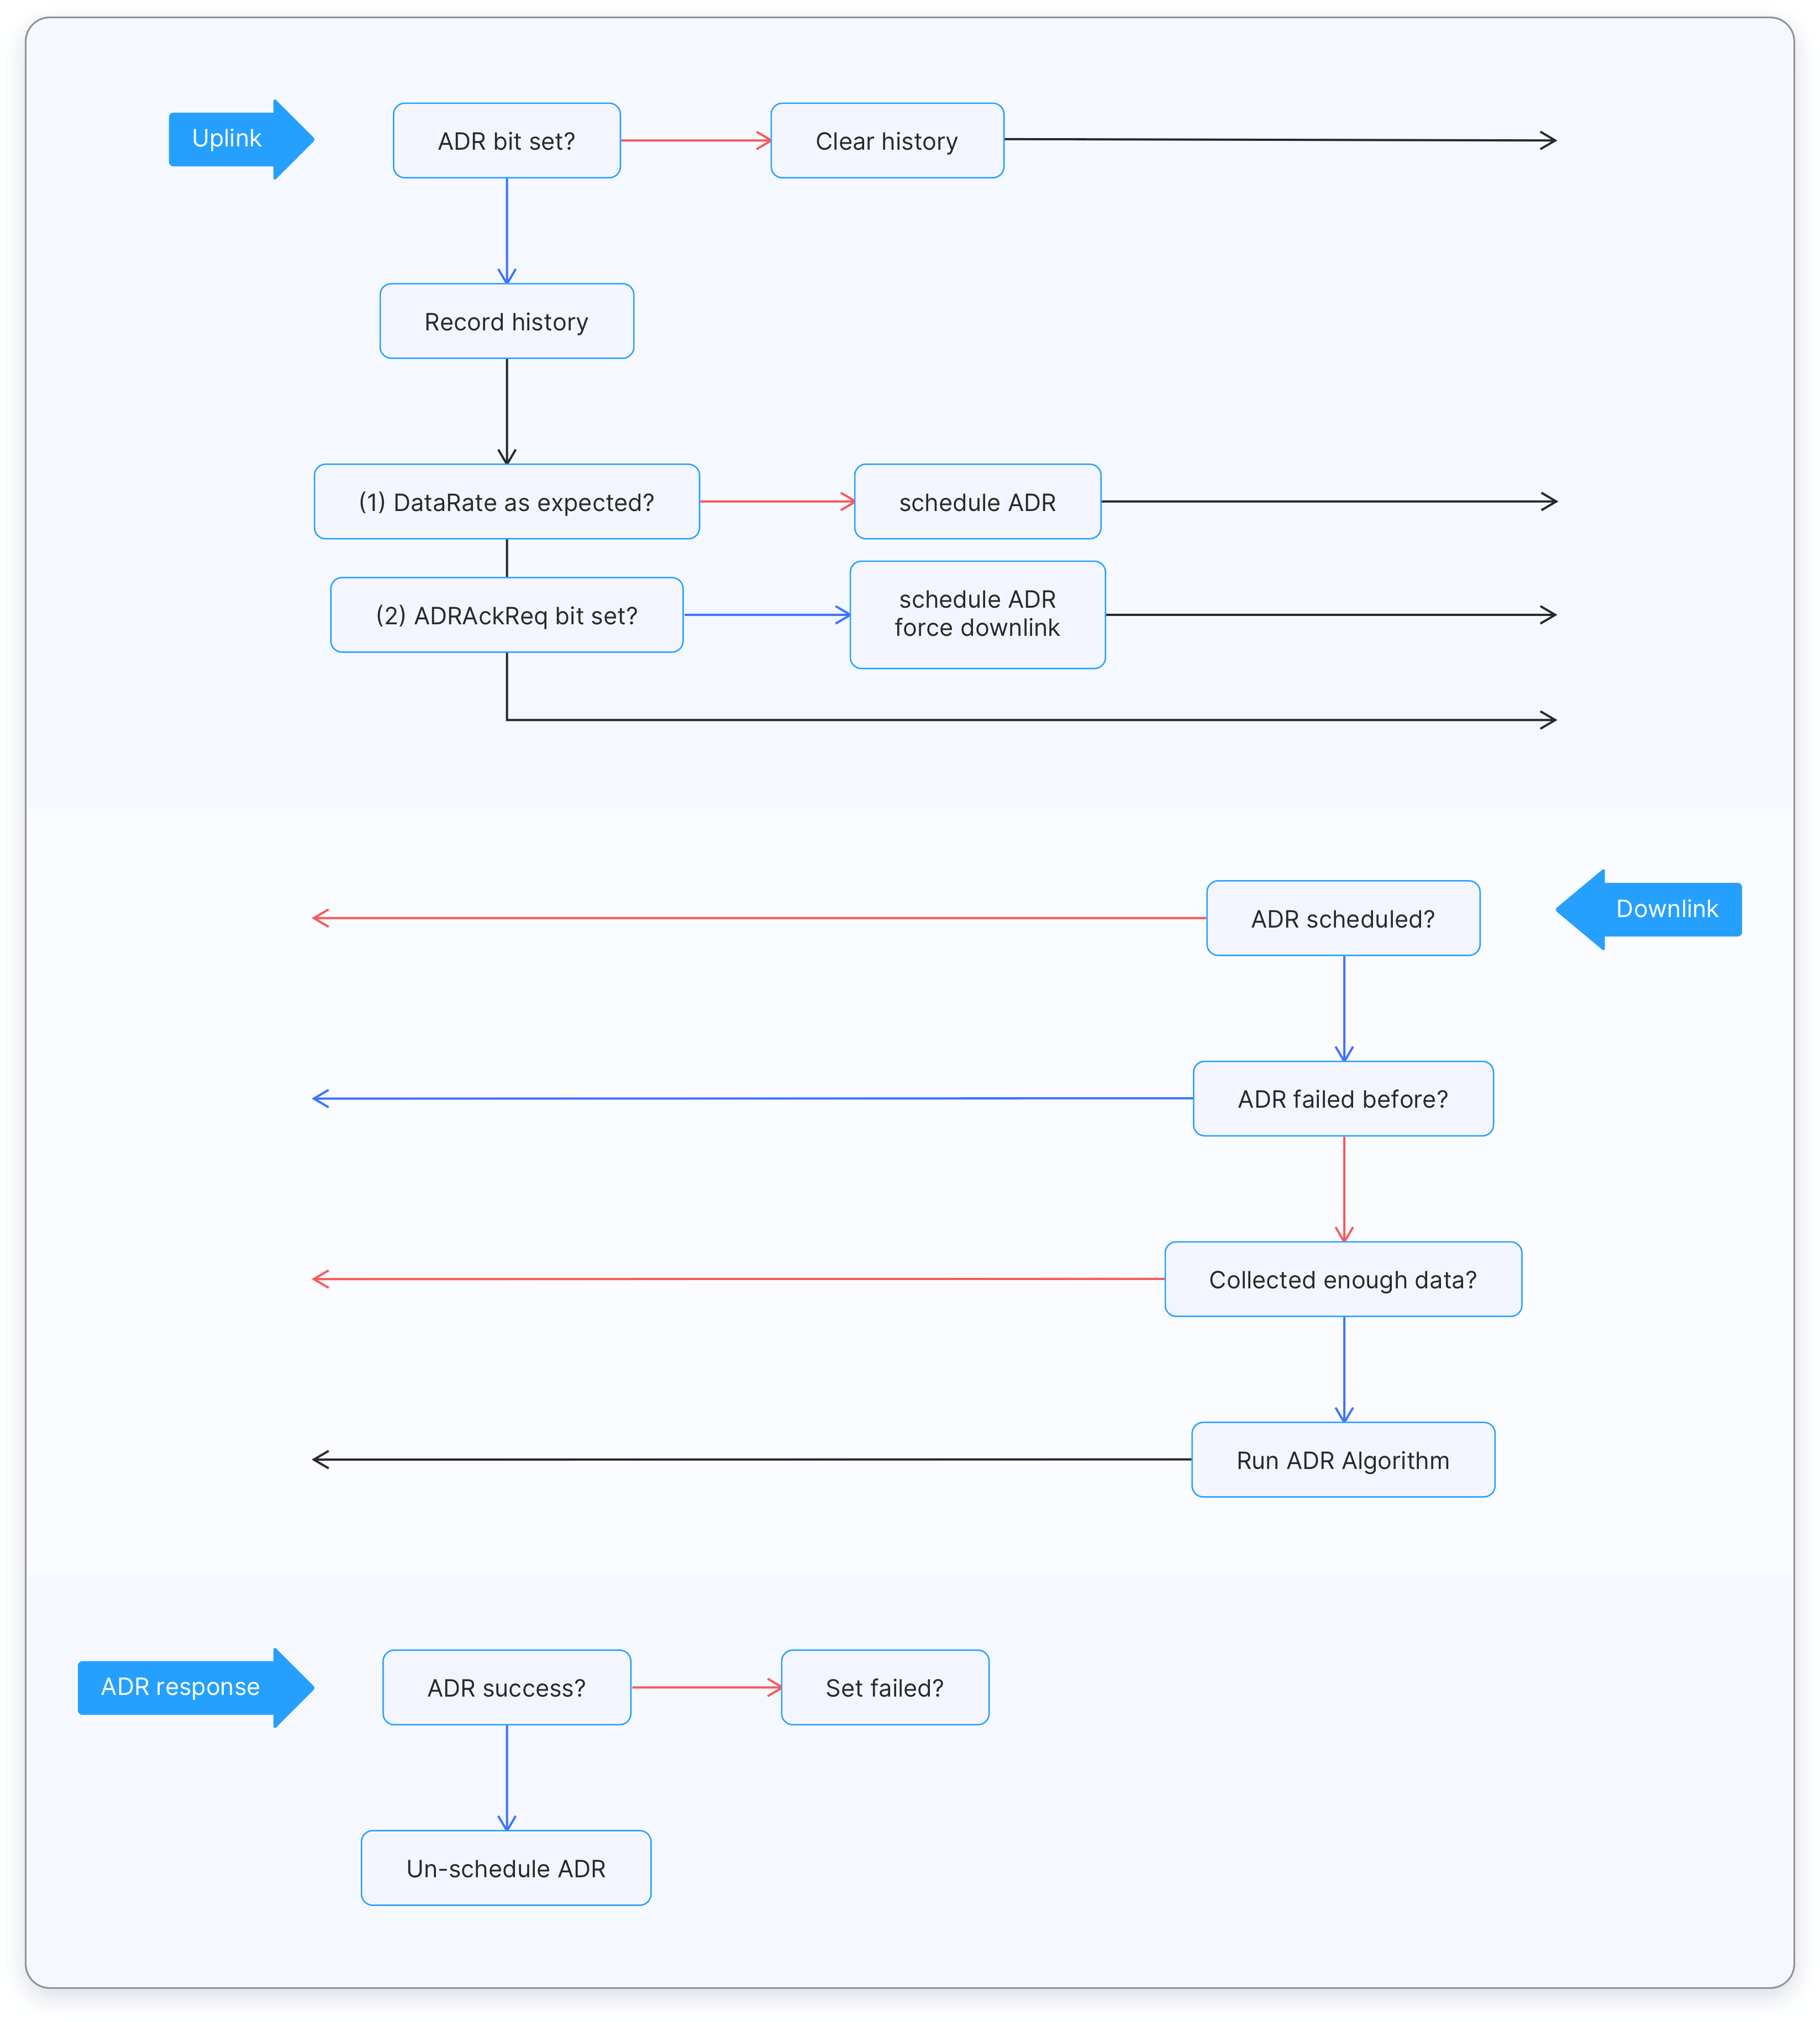
\includegraphics[width = \linewidth]{adr.png}
    \caption{Diagram outlines of the ADR flow in The Things Stack. More \href{https://www.thethingsnetwork.org/docs/lorawan/adaptive-data-rate/}{here}}
    \label{chap1:adr}
\end{figure}
\\
The ADR algorithm is the following:
\[
SNR_{margin} = SNR_{max} - SNR_{DR3} - margin_{dB}
\]
And with the SNRmargin we compute the steps up or down on DR/SF:
\[
Steps Up Or Down = \lfloor\frac{SNR_{margin}}{2.5}\rfloor
\]
As we take the maximum of the SNR of the past 20 packets, the 
performance of this algorithm is tuned for stationary nodes.
The TTN recommends the end node to have a fixed power and DR if the 
end node is movile. The obvious and worst case scenario where this algorithm would fail 
to give correct estimates is the one where the end node is moving away from 
the gateway. The first packet would be the maximum SNR, so the algorithm can not 
account for the decreasing SNR over the course of the next 19 received packets, 
resulting in a lower SF than what it would be needed in order to receive correctly 
in the future.\\



For any LPWAN technology it's crucial to incorporate security.
LoRaWAN uses two layers of security: one for the network layer and
another one for the application layer. The network security layer ensure
the authentication and all the transmission is encrypted by the
application layer with the AES method. Private session keys are needed
and there are two main different methods to obtain them:
\begin{itemize}
    \item[-] {\bfseries Over the air activation (OTAA):} in this method the device needs
to be equipped with a DevEUI that identifies the device, with a
AppEUI to identify the application and with a AppKey that is used
to sign an initial join request. Once the initial request is validated,
the join server generates the two session keys, and they are send
to the end node. Those keys are the NwSKey and the AppSKey
and are used to identify the network server and to encrypt the
payload.
    \item[-] {\bfseries Activation by personalization (ABP):} with this method you can
access the network without a join request because the device is
already equipped with the AppSKey and the NwSKey.
\end{itemize}
Usually the OTAA method is preferred, this is because it can generate
new session keys for each session and it allows re-key. ABP is not as
flexible as OTAA as the session keys are fixed in the device.
% add more sections and subsection here
% \subsection{Subsection One name}
% \label{sec:subsec11}

%%%%%%%%%%%%%%%%%%%%%%%%%%%%%%%%%%%%%%%%%%%%%%%%%%%%%%%%%%%%%%%%%%%%%%%%%%%%%%%%
%2345678901234567890123456789012345678901234567890123456789012345678901234567890
%        1         2         3         4         5         6         7         8
% THESIS CHAPTER

\chapter{Related Work}
\label{chap:second}
\ifpdf
    \graphicspath{{Chapter2/Figures/PNG/}{Chapter2/Figures/PDF/}{Chapter1/Figures/}}
\else
    \graphicspath{{Chapter2/Figures/EPS/}{Chapter2/Figures/}}
\fi

% short summary of the chapter
\section*{Summary}
% short summary of the chapter...

% One or more chapters should be devoted to the description of the
% proposed approach...

% In particular, this chapter describes the design adopted by this research to achieve the aims and objectives stated in the Introduction.
There have been studies conducted previously that aim to analyze parameters of lora communications in various enviroments, 
in this section we will see how they relate to our work and measurement results.\\

In the paper \cite{kousias2019empirical} the performance of ADR in a scenario in which the end nodes aren’t fixed is analized. 
The ED were following three different routes inside a truck with different speed. The authors found 
that as the mobility increase, the performance of the ADR starts to decrease leaving space for 
further improvements in the LoRaWan adaptative data rate.\\

The idea of paper \cite{benkahla2019enhanced} is to improve the ADR system used in LoRaWan and TTN for mobile ED. The E-ADR (enhanced ADR) 
they propose is based on transmit messages with the shortest possible time interval between them and to assume the 
trajectory of the mobile end-node. The results are impressive as they achieve to reduce the ToA and the energy 
consumption of the ED in the scenarios that are proposed. As a consequence, the packet loss is also reduced or 
eliminated because the achieved ToA minimizes the use of the allowed time limited by the duty cycle.\\

The authors in \cite{fargas2017gps} develop a system of geolocalization apart of gps or gsm based on the distance between the ED 
and the different gateways that is connected. They have reached an accuracy of 100m proving two different algorithms but it’s only a firs 
aproach as this method can’t be applied in real scenarios.


\label{sec:sa-temp}

%%%%%%%%%%%%%%%%%%%%%%%%%%%%%%%%%%%%%%%%%%%%%%%%%%%%%%%%%%%%%%%%%%%%%%%%%%%%%%%%
%2345678901234567890123456789012345678901234567890123456789012345678901234567890
%        1         2         3         4         5         6         7         8
% THESIS CHAPTER

\chapter{System architecture and hardware/software used}
\label{chap:third}
\ifpdf
    \graphicspath{{Chapter3/Figures/PNG/}{Chapter3/Figures/PDF/}{Chapter3/Figures/}}
\else
    \graphicspath{{Chapter3/Figures/EPS/}{Chapter3/Figures/}}
\fi


% short summary of the chapter
\section*{Summary}
% Discuss here the methodology used in the study, the stages by which the methodology was implemented, and the research design; For examples, one section details the participants in the study, another section lists all the instruments used in the study and justifies their use; another section outlines the procedure (algorithms, code,..) used; a section discusses how the data was analysed, etc..
In this chapter the design of our system is explained to give an
idea of how the idea of this project is applied to the TTN architecture.
In the other section we describe the devices and software used in order
to achieve the objective.

\section{Proposed system model}
\label{sec:s-system}
The next figure describes the proposed system in a graphical way to make it clear:
\begin{figure}[htbp]
    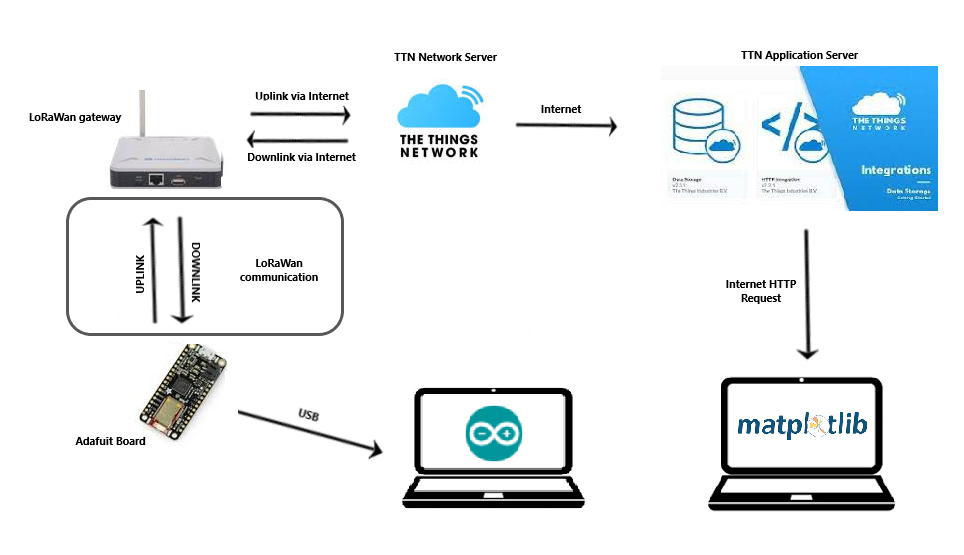
\includegraphics[width=\linewidth]{System.png}
    \caption{Proposed system}
\end{figure}

This LoRaWan system that is implemented starts with the laptop running the Arduino 
program on the adafruit board. The LoRaWan communication module of the board
is capable of transmitting LoRaWan packets to the gateway. This comunnication is the one 
in which the measurements will be taken, so is the one that will be analized in this thesis. 
The gateway is connected to the Internet via the operator networkand the data sent by the gateway 
will arrive first to the network server of TTN and then to our respective application server. 
The laptop is also making HTTP requests in order to analize the data from the database of the 
application server using python, specifically the library matplotlib. This architecture allows 
to analize the LoRaWan communication, which is the goal of this project.

\section{Devices used and their implementation}

\subsection{The gateway} 
\label{sec:s-gate}
The model of gateway used for this is the indoor Dragino lps-8. This device is forwarding LoRaWan 
packets via internet. This gateway acts like a bridge connecting the LoRaWan wireless network 
with the Internet. The indoor model was selected because in this case the gateway is fixed inside 
a building.
The gateway is on the 5$^{th}$ floor, connected to wall 
power through a USB-C port near a window in order to have the best possible . The access to the internet is 
provided through WiFi connection to the house router/modem. The configuration of the router was done 
as it is ilustrated in the figure \ref{chap:third:fig:gwconf}:

\begin{figure}[htbp]
    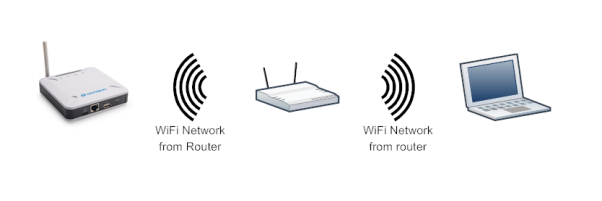
\includegraphics[width=\linewidth]{GatewayConfig.png}
    \caption{Configuration of the gateway via WiFi}
    \label{chap:third:fig:gwconf}
\end{figure}

On google maps, with a scale of 20 meters as shown in the image at figure \ref{sec:s-gw:loc}

The gateaway was located in the pinpoint shown in figure \ref{sec:s-gw:loc} 
\begin{figure}[htbp]
    \includegraphics[width=\linewidth]{mapaloragateway.png}
    \caption{Location of the gateway on the map}
    \label{sec:s-gw:loc}
\end{figure}


\section{The microcontroller}
\label{sec:s-micro}
The microcontroller used as a node in the network is the Adafruit Feather
M0 RFM95 LoRa Radio. The device is equipped with a transceptor
module LoRa, with built in USB and battery charging. The processor is
a ATSAMD21G18 ARM Cortex M0 at 48MHz and 3.3v (the same as the
Arduino Zero) and a quarter of a megabyte of FLASH, with 32k of RAM.
Thanks to the USB port, and a bootloader, the device can be
programmed and debugged through the USB port, no need for an
external programmer, which would have been yet another thin layer of
complexity.\\ 
\begin{figure}[htbp]
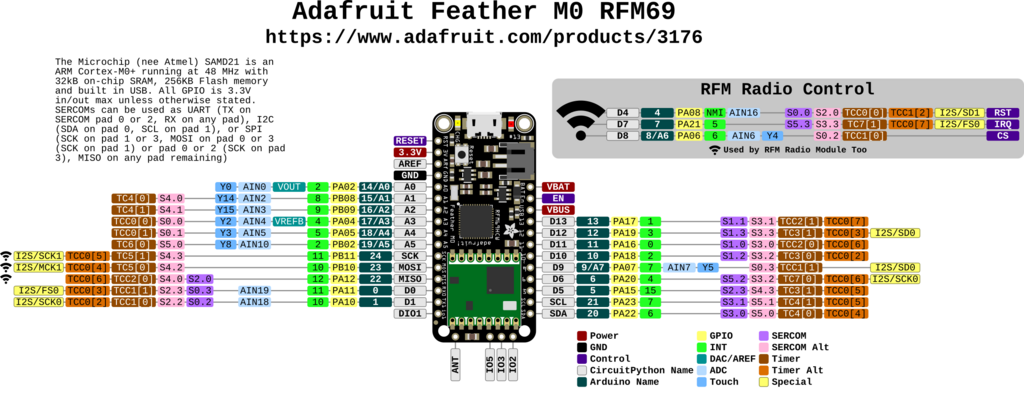
\includegraphics[width=\paperwidth, angle = 90]{pinout.png}
\caption{The pinout of the module}
\end{figure}
More info of the board and the pinout can be found \href{https://learn.adafruit.com/adafruit-feather-m0-radio-with-lora-radio-module/pinouts}{here}
The I2S connectors were used to connect the sensors which
communicated through the protocol, and DIO1 was manually wired to
GPIO6 so that the radio would work. For each individual sensor a different connection may be needed, so in
general, we connected the I2S to the same pins SCI and SDA and the
simple voltage for temperature sensor was connected directly to the
GPIO A0, setting it to an input on software to read from it.

\subsection{Sensors}
The first sensors mentioned were used to introduce us to the Arduino and IoT enviroment and the last one (the gps module)
is the one we finally used in order to measure the distance between the node and the gateway:
\begin{itemize}
    \item[-] Temperature and humidity sensors: 
        \begin{itemize}
        \item The \href{https://www.ti.com/lit/ds/symlink/hdc1080.pdf?ts=1655758883138&ref_url=https%253A%252F%252Fwww.google.com%252F}{hdc1080 sensor}
        is a digital humidity sensor with integrated temperature sensor that provide respective measurents using low power consumption.
        \item Another sensor with similar purpose is the \href{https://cdn-learn.adafruit.com/downloads/pdf/adafruit-bme280-humidity-barometric-pressure-temperature-sensor-breakout.pdf}{bme280 sensor}.
        in addition to the other one this sensor is capable of measuring preassure appart of temperature and humidity. 
        \end{itemize} 
        Two of this sensors were used and the respective models are hdc1080 bme280
    \item[-] Air quality sensor: sensor of the brand \code{SPEC SENSORS} specifically the model
    \href{https://www.spec-sensors.com/wp-content/uploads/2016/10/ULPSM-IAQ-968-008.pdf}{ULPSM-IAQ}. 
    It measures the indoor air quality   with very low power consumption and the output signal in this case is analog.

\end{itemize} 
This sensors are designed for the IoT enviroment as all of them use low power consumption. This characteristic is optimal 
for the purpose of LoRaWan networks using the less power consumption as possible. 

\subsection{GPS module and antenna}
The module \href{https://www.u-blox.com/en/product/lea-6-series}{u-block LEA-6S-0-001} 
is able to obtain the specific coordinates in which the module is placed with a precission of 2.5m and 
it's also designed for low power consumption. \\

This module is designed for the use of passive and active antenna. The antenna selected for this gps module is an 
active one, which means that the received signal is amplified. The available freaquency bands are the following ones:

\begin{figure}
    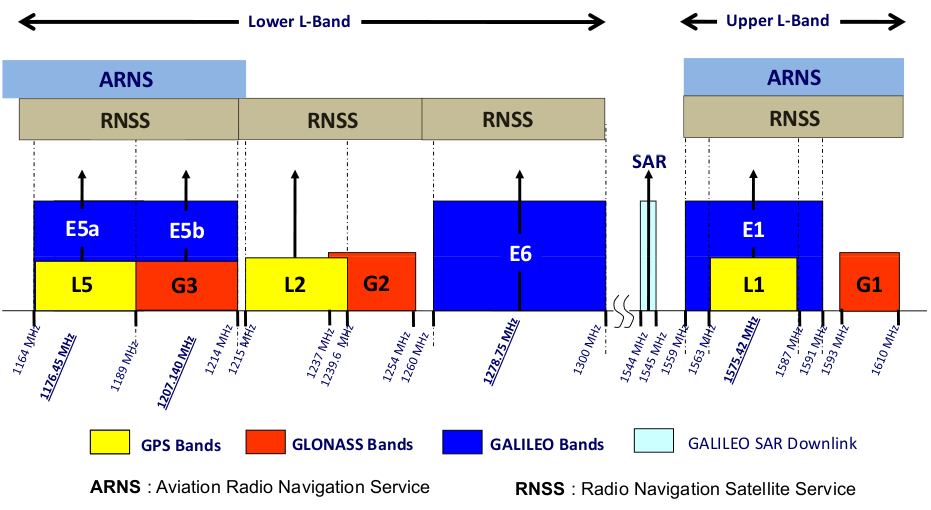
\includegraphics[width = \linewidth]{GPS_frequency_bands.png}
    \caption{Center frecuency and BW for the three different GPS bands}
\end{figure}

In our case we will work with 1575 MHz as it is the band that detects our antenna.



\section{Software used}
\label{sec:s-m-soft}

\subsection{MCCI LMIC Arduino library}
\label{sec:s-m-lmic}

The \code{MCCI\_LoRaWAN\_LMIC} library was the most complete library for
our purpose. The recommended library by Adafruit has the flaw of not
being compliant with the TTN standard anymore as it cannot receive
downlink messages, and the RadioHead library is a LoRa library,
requiring us to implement the whole LoRaWAN engine for ourselves.
\code{MCCI\_LoRaWAN\_LMIC} library is already done so there was no need to
waste our efforts. For more information about the library, the
documentation, code and repository are 
\href{https://github.com/mcci-catena/arduino-lmic.}{here}. The library is a pretty big and complex piece of C code, so a brief
explanation will be given.
Using the 4.1.0 version, so it will be the model explained:
(GPS Click - Breakout Board for u-blox LEA-6s, 2022)

\begin{figure}[htbp]
\centering
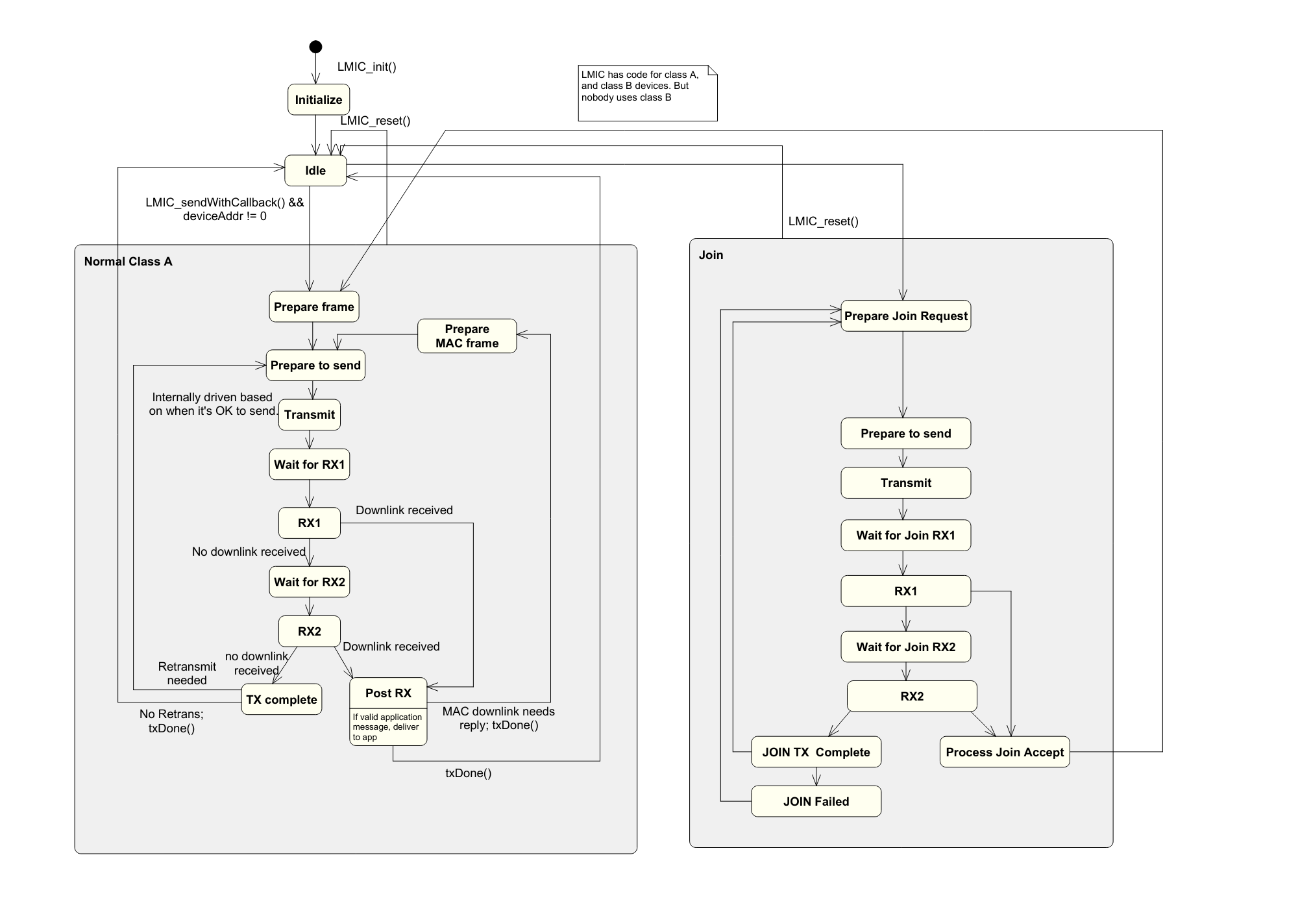
\includegraphics[width=\paperwidth, angle= 90]{modelLMIC.png}
\caption{Finite state machine of LMIC library}
\label{sec:lib-finitestate}
\end{figure}
In figure \ref{sec:lib-finitestate} is pictured the whole finite state machine. The only part a user should be
concerned about is the frame data set up, the actions to be taken for
every event desired to react to with the \code{onEvent()} call-back function
or \code{LMIC\_registerEventCb()} API function. Both are currently
supported, and although the \code{onEvent()} application call-back is
currently deprecated, it still works on version 4 and it is simple to
implement and debug. The other option is the recommended one, but is
harder to comprehend.
We ended with a function that, when the package is sent, a timed call-
back is issued thanks to the convenience function
\code{os\_setTimedCallback()} to schedule a job in the next
\code{TX\_INTERVAL}, that job in charge of queuing up another packet of data
to be sent, witch will be collected by the engine and, when sent, the cycle
starts once again: \\
first job → sent → wait TX → job → sent → wait TX → job ... \\
This is “interrupted” by the compliance engine, that ensures that
the law is not broken by keeping track of the air time so that the device
can't send more than the percentage set by the region configuration in the library
(currently on EU 868).
The I2C library was used to communicate with the sensors, as a
dependency of the particular libraries for each one of them.
\code{ClosedCube\_HDC1080} library was used for the more straightforward
and the \code{Adafruit\_BME280} was used for the other sensor.

\subsection{TinyGPSPlus}
\label{sec:s-m-tinygps}
This library is design to parse all type of NMEA data that the GPS module provides. In our case this 
library is used in order to extract the exact latitude and longitude of the ED. More info about this 
library can be found in the \href{https://github.com/mikalhart/TinyGPSPlus}{github repository}

\subsection{U-center}
\label{sec:s-m-ucenter}
The software developed by the company u-block is a monitoring system for the gps module mentioned before. 
U-center provides info about the signal that gps is detecting from the gps-satellites. Once the gps is 
calibrated the u-center software provides all data the gps is collecting including the longtude and latitude.

\subsection{Arduino}
\label{sec:s-m-lmic}

\subsection{Python}
\
%%%%%%%%%%%%%%%%%%%%%%%%%%%%%%%%%%%%%%%%%%%%%%%%%%%%%%%%%%%%%%%%%%%%%%%%%%%%%%%%
%2345678901234567890123456789012345678901234567890123456789012345678901234567890
%        1         2         3         4         5         6         7         8
% THESIS CHAPTER

\chapter{Experimental Results
}
\label{chap:er1}
\ifpdf
    \graphicspath{{Chapter4/Figures/PNG/}{Chapter3/Figures/PDF/}{Chapter4/Figures/}}
\else
    \graphicspath{{Chapter4/Figures/EPS/}{Chapter3/Figures/}}
\fi


% short summary of the chapter
\section*{Summary}
Details all the results of your study here (exploits graphics for results visualization). 
This chapter should also contain a full discussion, interpretation and evaluation of the results. 



\section{Section 1} 
\label{sec:gv2}


%%%%%%%%%%%%%%%%%%%%%%%%%%%%%%%%%%%%%%%%%%%%%%%%%%%%%%%%%%%%%%%%%%%%%%%%%%%%%%%%
%2345678901234567890123456789012345678901234567890123456789012345678901234567890
%        1         2         3         4         5         6         7         8
% THESIS Chapter
\chapter{Data analysis for first and second experiments}
\label{chap:fifth}
\ifpdf
    \graphicspath{{Chapter5/Figures/PNG/}{Chapter5/Figures/PDF/}{Chapter5/Figures/}}
\else
    \graphicspath{{Chapter5/Figures/EPS/}{Chapter5/Figures/}}
\fi

In this section the graphs are displayed, whereas in \ref{chap:conclusions} this will be 
explained. For the second experiment the parsed json structure was used to simplify the 
representation of the data with python.
\section{Results of the first experiment}
The packet structure for the first experiment is as follows:

\begin{minted}{json}
    {
        "powRet": 17,
        "f_port": 42,
        "f_cnt": 51,
        "rssi": -90,
        "rssi_ch": -90,
        "snr": 4.8,
        "bw": 125000,
        "SF": 7,
        "f(MHz)": 867.5,
        "time": "YYY-MM-DDTHH:mm:ss.ssssss+HH:mm",
    }
\end{minted}


The tables for losses on the first experiment are included, but for the second, the tables are on 
 chapter \ref{chap:conclusions} \\
\begin{figure}[htbp]

    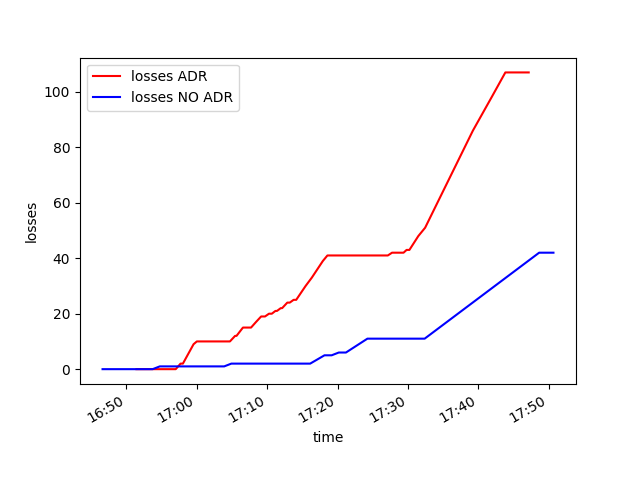
\includegraphics[width=\linewidth]{losses.png}
    \caption{Acummulative packet loss depending on the time the packets arrived}
    \label{chap:fifth:fig:1}
\end{figure}

\begin{figure}[htbp]
    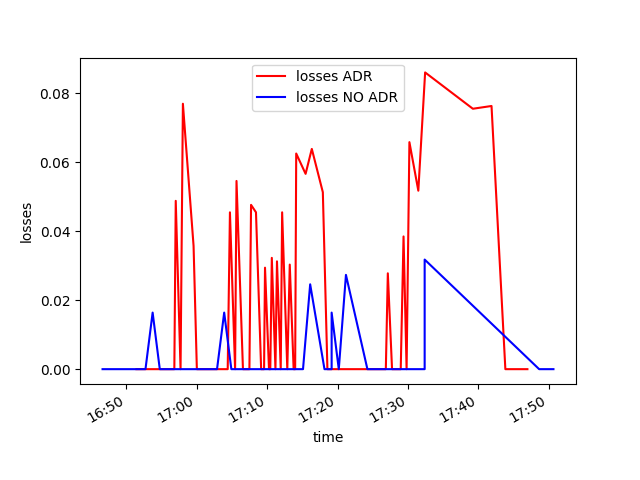
\includegraphics[width=\linewidth]{lossesderivadas.png}
    \caption{The discrete derivative of \ref{chap:fifth:fig:1}}
    \label{chap:fifth:fig:3:noADR}
\end{figure}

\begin{figure}[htbp]
    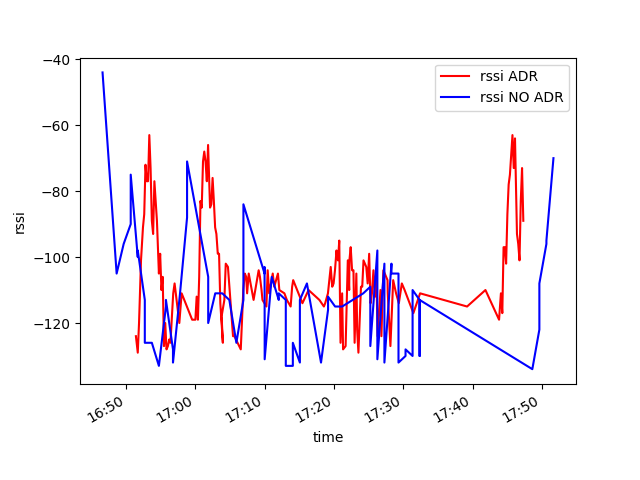
\includegraphics[width=\linewidth]{RSSI.png}
    \caption{RSSI depending on the time}
    \label{chap:fifth:fig:2}
\end{figure}



\begin{table}[htpb]
    \centering
    \setlength{\arrayrulewidth}{0.5mm}
    \setlength{\tabcolsep}{18pt}
    \renewcommand{\arraystretch}{2}
    \begin{tabular}{|c|c|c|c|}
        \hline
         \cellcolor[HTML]{85C1E9}ED configuration & \cellcolor[HTML]{85C1E9}Packets sent & \cellcolor[HTML]{85C1E9}Packets received & \cellcolor[HTML]{85C1E9}Packet loss\\
         \hline
         ADR activated & 263 & 156 & 40.68\% \\
         SF10 and 14 dBm & 112 & 70 & 37.5\% \\
         \hline
    \end{tabular}
    \caption{Table comparing the packet loss of the two cases}
    \label{tab:packet_loss_exp1}
\end{table}

\begin{table}[htbp]
    \centering
    \setlength{\arrayrulewidth}{0.5mm}
    \setlength{\tabcolsep}{18pt}
    \renewcommand{\arraystretch}{2}
    \begin{tabular}{|c|c|c|}
        \hline
         \cellcolor[HTML]{85C1E9}ED configuration & \cellcolor[HTML]{85C1E9}Medium SNR (dB) & \cellcolor[HTML]{85C1E9}Medium RSSI (dBm)\\
         \hline
         ADR activated & 2.07 & -103.68 \\
         SF10 and 14 dBm & -2.11 & -111.85 \\
         \hline
    \end{tabular}
    \caption{Table comparing the medium RSSI and SNR in both cases}
    \label{tab:RSSI_SNR_exp1}
\end{table}


\section{Results of the second experiment}
Our parsed package structure is the following:\\

\begin{minted}{json}
    {
        "powRet": 17,
        "f_port": 42,
        "f_cnt": 51,
        "rssi": -112,
        "rssi_ch": -112,
        "snr": 4.8,
        "bw": 125000,
        "SF": 7,
        "f(MHz)": 867.5,
        "time": "YYY-MM-DDTHH:mm:ss.ssssss+HH:mm",
        "lat": 44.4134407043457,
        "lng": 8.928983688354492
    }
\end{minted}
This was downloaded and parsed from the storage integration The Things Network provides.
It is suitable for us, since we do not need instant feedback, for that we would have to 
set up a webhook on an external server. The date is on ISO format. 
From here we parse the graphs depicted on chapter \ref{chap:conclusions}.


%%%%%%%%%%%%%%%%%%%%%%%%%%%%%%%%%%%%%%%%%%%%%%%%%%%%%%%%%%%%%%%%%%%%%%%%%%%%%%%%
%2345678901234567890123456789012345678901234567890123456789012345678901234567890
%        1         2         3         4         5         6         7         8
% THESIS CONCLUSIONS
\def\baselinestretch{1}
\chapter{Conclusions}
\label{chap:conclusions}
\ifpdf
    \graphicspath{{Conclusions/Figures/PNG/}{Conclusions/Figures/PDF/}{Conclusions/Figures/}}
\else
    \graphicspath{{Conclusions/Figures/EPS/}{Conclusions/Figures/}}
\fi
\def\baselinestretch{1.0}

% quote

Conclusions should summarize the problem, the solution and its main innovative features, outlining future work on the topic or application scenarios of the proposed solution.


%%%%%%%%%%%%%%%%%%%%%%%%%%%%%%%%%%%%%%%%%%%%%%%%%%%%%%%%%%%%%%%%%%%%%%%%%%%%%%%%
%2345678901234567890123456789012345678901234567890123456789012345678901234567890
%        1         2         3         4         5         6         7         8
% THESIS APPENDIX

\chapter{Gesture Vocabulary} 
\label{chap:appendixA}


\begin{figure}
    \centering
    \includegraphics[width=0.8\textwidth]{Chapter4/Figures/Figures/gv.PNG}
    \caption{Proposed gesture vocabulary}
    \label{fig:gs}
\end{figure}


\appendix
%%%%%%%%%%%%%%%%%%%%%%%%%%%%%%%%%%%%%%%%%%%%%%%%%%%%%%%%%%%%%%%%%%%%%%%%%%%%%%%%%
%2345678901234567890123456789012345678901234567890123456789012345678901234567890
%        1         2         3         4         5         6         7         8
% THESIS APPENDIX

\chapter{Gesture Vocabulary} 
\label{chap:appendixA}


\begin{figure}
    \centering
    \includegraphics[width=0.8\textwidth]{Chapter4/Figures/Figures/gv.PNG}
    \caption{Proposed gesture vocabulary}
    \label{fig:gs}
\end{figure}


%\chapter{Survey}
\label{chap:appendixB}


%\begin{figure}
%\setboolean{@twoside}{false}
% Uncomment the follow line to show the survey
\includepdf[pages=1-,scale=0.8,pagecommand={}]{Appendix2/gbhri3_format.pdf}
%\end{figure}

%\begin{figure}
 %\centering 
 %\includegraphics{Appendix2/gbhri3_format.pdf}
%\end{figure}
%\bibliographystyle{Classes/RoboticsBiblio}    % bibliography style
\bibliographystyle{ieeetr}
\renewcommand{\bibname}{References}           % change default name Bibliography to References
\bibliography{References/references}          % References file
\addcontentsline{toc}{chapter}{References}    % add References to contents page
%\addcontentsline{toc}{section}{References}
\nocite{*}
\end{document}
